\section{Техническое задание}
\subsection{Основание для разработки}

Основанием для разработки является задание на выпускную квалификационную работу бакалавра "<Разработка web-сайта \textquotedbl Русатом -- Аддитивные технологии\textquotedbl\ на платформе 1С-Битрикс">.

\subsection{Цель и назначение разработки}

Основной задачей выпускной квалификационной работы является разработка и внедрение web-сайта для продвижения компании ООО «Русатом – Аддитивные технологии».

Посредством внедрения web-сайта планируется устранить существующие недостатки в компании. Исходя из этого, основную цель предлагается рассмотреть в разрезе двух групп подцелей.

Задачами данной разработки являются:
\begin{itemize}
\item создание информационных разделов сайта;
\item    реализация формы для обратной связи;
\item реализация калькулятора расчета стоимости изготовления деталей;
\item реализация формы заявки на изготовление деталей;
\item создание удобного поиска по сайту.
\end{itemize}

\subsection{Требования пользователя к интерфейсу web-сайта}

Сайт должен включать в себя:
\begin{itemize}
    \item навигацию по разделам;
    \item авторизацию;
    \item доступы для администратора, редактора, исполнителя по заявкам с форм.
\end{itemize}

Композиция шаблона сайта представлена на рисунке ~\ref{templ:image}.

\begin{figure}[h]
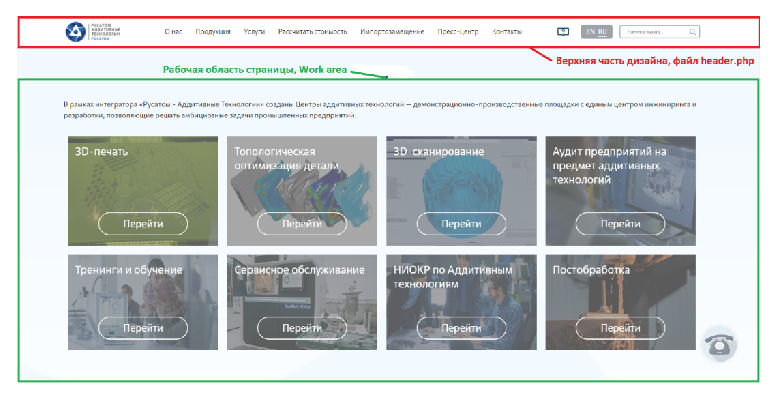
\includegraphics[width=1\linewidth]{templ}
\caption{Композиция шаблона сайта}
\label{templ:image}
\end{figure}
%\vspace{-\figureaboveskip} % двойной отступ не нужен (можно использовать, если раздел заканчивается картинкой)

\subsection{Моделирование вариантов использования}

Для разрабатываемого сайта была реализована модель, которая обеспечивает наглядное представление вариантов использования сайта.

Она помогает в физической разработке и детальном анализе взаимосвязей объектов. При построении диаграммы вариантов использования применяется унифицированный язык визуального моделирования UML.

Диаграмма вариантов описывает функциональное назначение разрабатываемой системы. То есть это то, что система будет непосредственно делать в процессе своего функционирования. Она является исходным концептуальным представлением системы в процессе ее проектирования и разработки. Проектируемая система представляется в виде ряда прецедентов, предоставляемых системой актерам или сущностям, которые взаимодействуют с системой. Актером или действующим лицом является сущность, взаимодействующая с системой извне (например, человек, техническое устройство). Прецедент служит для описания набора действий, которые система предоставляет актеру.

На основании анализа предметной области в программе должны быть реализованы следующие прецеденты:
\begin{enumerate}
\item Просмотр информации о компании.
\item Просмотр информации о продукции компании.
\item Просмотр информации об услугах компании, много услуг, длинный список, не поместится никак в одну строку.
\item Поиск по сайту.
\end{enumerate}

\subsection{Требования к оформлению документации}

Разработка программной документации и программного изделия должна производиться согласно ГОСТ 19.102-77 и ГОСТ 34.601-90. Единая система программной документации.
